%% Version 3/21/02
%%%%%%%%%%%%%%%%%%%%%%%%%%%%%%%%%%%%%%%%%%%%%%%%%%%%%%%%%%%%%%%%
%% Kluwer Edited Book Template File, Edbktmpl.tex
%%
%% Kluwer Academic Press
%%
%% Prepared by Amy Hendrickson, TeXnology Inc., July 1999.
%%%%%%%%%%%%%%%%%%%%%%%%%%%%%%%%%%%%%%%%%%%%%%%%%%%%%%%%%%%%%%%%

%%%%%
%% LaTeX2e
%% Uncomment documentclass,
\documentclass{kapedbk} % Computer Modern font calls

%% and, optionally, one or more
%%   of the \usepackage commands below:

%%%%%
%% If you use a font encoding package, please enter it here, i.e.,
%  \usepackage{T1enc}

%%%%%
%  If you have MathTimes and MathTimesPlus fonts, you
%  may uncomment the line below and use them, but you are
%  not obligated to do so, and most authors do not have
%  these fonts. (You may need to edit m-times.sty to make the
%  font names match those on your system)

%  You must have the MathTimes fonts for this to work. They may be
%  purchased from the Y&Y company, http://www.YandY.com.

% \usepackage[mtbold,noTS1]{m-times}

%%%%%
% PostScript font calls
%
% If you use the edbkps.sty font file, you may need to edit it
% to make sure the font names match those on your system. See
% the top of the edbkps.sty file for more info.

\usepackage{edbkps}

%%%%%
% Style for inserting .eps files and rotating illustrations or tables

% possible options for graphicx:
% [dvips], [xdvi], [dvipdf], [dvipsone], [dviwindo], [emtex], [dviwin],
% [pctexps],  [pctexwin],  [pctexhp],  [pctex32], [truetex], [tcidvi],
% [oztex], [textures]

\usepackage[dvips]{graphicx}

%%%%%%%%%%%%%%%%%%%%%
%% LaTeX209,
%  Uncomment only one below, comment out similar commands above
%  \documentstyle{kapedkbk} % Computer Modern fonts
%  \documentstyle[edbkps]{kapedbk} %For PostScript fonts
%  (The m-times.sty works only with LaTeX2e)

%%%%%%%%%%%%%%%%%%%%%%%%%%%%%%%%%%%%%%%%%%%%%%%%%%%%%%%%%%%%%%%%%%%%%%%%%
%% Commands You Can Set or Change to Customize Your Book Format: ===>>>

% Running heads:
% ==============

%  Uncomment to make chapter title on left hand page
%  and section title on right hand page
%  \chapsectrunningheads


% Section heads:
% ==============

%%%
% \chaptersection % will use chapter.section form for section heads.

%%%
% Uncomment to make section heads appear in
%                    both upper and lower case.
%\upperandlowercase

\useuppercase % Uncomment to make section and subsection heads
              %  appear in uppercase.

%%%
% How many levels of section head would you like numbered?
% 0= no section numbers, 1= section, 2= subsection, 3= subsubsection
\setcounter{secnumdepth}{2}

% Table of Contents:
% ==================
% How many levels of section head would you like to appear in the
%  Table of Contents?
%  0= chapter titles, 1= section titles, 2= subsection titles,
%  3= subsubsection titles.

\setcounter{tocdepth}{1}

% Equation numbering:
% ===================

%%%
% \nochapequationnumber % will result in equation numbers that are (1)

%%%
% \sectionequationnumber % will result in equation numbers that are (1.1)
                         % and renumber for each section

% Default for kapedbk is (chapternumber.equationnumber)
% Default for kapproc is (equation number)

% Theorem numbering:
% ==================
% \nochaptheoremnumber % will make the theorem type environments number
       % only with the theorem number. Default is chapter.theorem for
       % kapedbk.

% Footnotes/Endnotes:
% ===================

% Default is endnotes that appear at the end of the chapter, above
% the references, or whereever \notes is written.

%%%
% To change footnotes to appear at bottom of page uncomment:
% \let\footnote\savefootnote

%%%
% Uncomment if you want footnotetext to appear at the bottom of the page:
%\let\footnotetext\savefootnotetext

%%%
% Uncomment if you want a ruled line above the footnote.
%\let\footnoterule\savefootnoterule

% Bibliography Style Settings:
% ============================
% Choose either kluwerbib or normallatexbib:

%%%
%\kluwerbib % will produce this kind of bibliography entry:

%  Anderson, Terry L.,...
%    continuing bib entry here

%  \cite{xxx} will print without brackets around the citation.
% \bibliographystyle{kapalike} % should be used when you use \verb+\kluwerbib+.

%%%
\normallatexbib %will produce bibliography entries as shown in the
                % LaTeX book

% [1] Anderson, Terry L.,
%     continuing bib entry

% \cite{xxx} will print with square brackets around the citation, i.e., [1].

% Any \verb+\bibliographystyle{}+ may be used with \verb+\normallatexbib+, but
% you should check with your editor to find the style preferred for
% your book.

% Change Brackets around Citation:
% ================================

%% Default with \kluwerbib is no brackets around citation.
%% Default with \normallatexbib is square brackets around citation.

% For parens around citation uncomment these:

%\let\lcitebracket(
%\let\rcitebracket)

% For square brackets around citation uncomment these:

%\let\lcitebracket[
%\let\rcitebracket]

% Draft Line:
% ===========
%  Optional, uncomment to make current time and `draft' appear at
%  bottom of page.

%\draft

%%%% <<== End Formatting Commands You Can Set or Change %%%%%%%%%%%%%%%%%
%%%%%%%%%%%%%%%%%%%%%%%%%%%%%%%%%%%%%%%%%%%%%%%%%%%%%%%%%%%%%%%%%%%%%%%%%

\usepackage{comment}
\usepackage{url}

\newif{\ifTODO}
% utiliser l'une ou l'autre de ces commandes
%  \TODOtrue   
%  \TODOfalse  
\newcommand{\todo}[1]{\ifTODO{\marginpar{$`[:-]$}{[[\small #1]]}} \else{} \fi}
\newif{\ifTADA}
% utiliser l'une ou l'autre de ces commandes
%  \TADAtrue   
%  \TADAfalse  
\newcommand{\tada}[1]{\ifTADA{\marginpar{$`[:-]`[:-]$}{[[\small #1]]}} \else{} \fi}
\newcommand{\done}[1]{\marginpar{$\smiley$}{[[\small #1]]}}

\newcounter{acommentcounter}

\newif{\ifTOREMOVE}
\newcommand{\toremove}[1]{\ifTOREMOVE{\marginpar{\tiny to remove ?}{\textbf{#1}}} \else{} \fi}

\newif{\ifENABLECOMMENT}
\newcommand{\acomment}[2]{\ifENABLECOMMENT{
	\addtocounter{acommentcounter}{1}
	\marginpar{\small [*\arabic{acommentcounter}]#1 }{\textbf{[*\arabic{acommentcounter}]#2}}} \else{} \fi}


\ENABLECOMMENTtrue
\TOREMOVEtrue

\def\e{{\it e}}
\def\scarie{{SCARI\e}}
\def\das3{\mbox{DAS-3}}
\def\evlbi{{\it e}-VLBI}


%%%%%%%%%%%%%%%%%%%%%%%%%%%%%%%%%%%%%%%%%%%%%%%%%%%%%%%%%%%%%%%%%%%%%

\begin{document}


%------ article title  ------------------->>

% If you use \\'s , please supply an alternate version of the title
% in square brackets, i.e.,
%\articletitle[Communism, Sparta, and Plato]
%{COMMUNISM, SPARTA,\\ and PLATO}
%\articletitle{Towards Real-time Software Correlation on Grids.}
\articletitle{Real-time Software Correlation.}

%% optional, to supply a shorter version of the title for the running head:
%\chaptitlerunninghead{Eventual other Running Head}

%\articlesubtitle{Eventual Subtitle}
%\vspace{-0.36cm}

\author{Nico Kruithof\altaffilmark{1}, Damien Marchal\altaffilmark{2}}
\affil{\altaffilmark{1} Joint Institute for VLBI in Europe (JIVE),
  Postbus 2, 7990 AA Dwingeloo, The Netherlands
\mbox{Kruithof@jive.nl}, \\
\altaffilmark{2} University of Amsterdam (UvA),
Kruislaan 403, 1098 SJ Amsterdam, The Netherlands
\mbox{dmarchal@science.uva.nl}
}

\begin{abstract}
  In this paper we present the progress of the \scarie\ project. In
  which, we investigate the capabilities of a next generation
  grid based software correlator for VLBI. We will mostly focus on the
  current design of our software correlator, and on the challenges of
  running real-time scientific experiments on top of grids
  infrastructure. This paper also contains experimental results on
  both software correlation as well our current experiments on the
  DAS-3 grid and StarPlane its user-controllable dynamic photonic
  network.
\end{abstract}

%\begin{keywords}
%Eventual keywords
%\end{keywords}


\vspace{0.64cm}
\section{Introduction}
\begin{comment}
  Very Long Baseline Interferometry (VLBI) \cite{VLBIbook} is a type of
  interferometry used in radio astronomy, in which data received at
  several telescopes is combined to produce an image with very high
  resolution. VLBI can be used for both astronomy and geodesy.  For
  astronomy, VLBI provides high-resolution images of radio sources in
  the sky, whereas in geodesy VLBI measures the location of the
  telescopes and the Earth Orientation Parameters (EOP).
\end{comment}

Recent Astronomical researches aims to study the deep-sky (farther and
farther away from us) which requires higher and higher angular
resolution to capture all the details of the observed sources.
Increasing the size of a telescope dish increases the increase the
angular resolution of the image linearly.  Nevertheless, due to
mechanical constraints, it is difficult to build moveable telescope
dishes with a size much larger than 100m. Interferometry provides a
possible solution to this problem as it permit to combine the
measurements of several telescopes to simulate a dish of size
equivalent to the maximal distance between the farthest telescopes.
This approach is called Very Large Baseline Interferometry (VLBI) and
permits us to build a virtual telescope with a dish of a size of the
earth (or more). Once the data has been recorded, the data of each
pair of stations has to be correlated.  In the \scarie\ project we are
developing and analyzing the capabilities of making a software
correlator that uses the processing power of a grid.

\scarie\ is a typical example of a recent trend of the e-Science 
community in which computation resources and scientific instruments 
are connected worldwide through high-speed networks. We think that to 
generalize the utilization of such world-size inter-connected facility, 
the grids and their middlewares have to offer services that matches the three
following user-application requirements:
\begin{itemize}
\item \emph{better performances}: an application is said performance
  limited if the resources needed to run it are not large enough to
  satisfy its needs. Performance limitations can have multiple
  origins: insufficient computing resources, memory, high network
  latency or low network throughput.
  
\item \emph{isolated environment}: there are classes of applications
  that can only be executed if put in an isolated environment in the 
  sense that the other users'application cannot interfere. Examples are 
  real-time distributed application, or benchmarks that require reproducible
  result. 

\item \emph{scheduling}: some application requires to be synchronized
  with "external events" (like having radio-telescope looking at a
  specific location in the sky at a specific date). In order to
  execute such application it is mandatory to schedule its execution 
  and reserve the needed resource in advance.
\end{itemize}
In order to fully reach the \scarie\ objectivs these three 
requirements have to be addressed for networking resource, nodes and 
data space. These are still hot-topics in the grid communauty, 
especially because networking has a long history as a 
\emph{best-effort} shared resourced which is incompatible 
with an isolated network environment. For this reason we are 
conducting ours experiences using the experimental \das3\ 
grids as it have an user-controllable dynamic photonic 
network called StarPlane to build, on demand and application specific, 
isolated virtual-network on top of the complete grid. A such service would 
permit to run \scarie\ with a good confidence level that a real-time 
experiment will not be disturbed by other users. \\

The rest of the paper is organized as follows. Section~\ref{sec:vlbi}
contains a general introduction to VLBI and its recent development 
called \evlbi. Section~\ref{sec:softwarecorrelation} describes the 
architecture of the software correlator. Section~\ref{sec:network} 
describes how the software correlator make use of the StarPlane services 
and the \das3 resources. We present benchmarks in Section~\ref{sec:benchmarks} 
and conclude the paper with future work in Section~\ref{sec:conclusion}.


\section{VLBI}\label{sec:vlbi}
In order to approximate a telescope with a larger dish, multiple
telescopes can observe the same object, and the data can be combined
using interferometry. The angular resolution of the VLBI array of
telescopes depends on the maximal projected distance between two
telescopes, while the sensitivity depends on the number of telescopes
and the bandwidth. To acquire high sensitivity data rates upto 1Gbs
per telescope are used.  The requirements on both the data streams and
the computing power to achieve a good sensitivity are shown in
Table~\ref{tab:speed}.

Traditionally, the data is recorded at the telescopes on
disk packs during a VLBI experiment. After the experiment the disks
are shipped to a central institute, e.g. the Joint Institute for VLBI
in Europe (JIVE), for correlation. At JIVE, the data from the
different telescopes is read from the disks and correlated by a
dedicated hardware correlator~\cite{EVNCorrelator}. The maximal
capacity of this hardware correlator is 16 telescopes at a data rate
of 1Gbs each.  There can be several weeks between the experiment and
the time when the correlated data becomes available.

% \marginpar{NGHK: Check 16Mb/s in table}
\begin{table}
  \centering
  \begin{tabular}[c]{|l|l|l|l|l|l|}
    \hline
    Description & \# & \#  & data-rate & spect/prod & Tflops\\
    & telescopes & sub-bands & (Mb/s) &  & \\
    \hline
    \hline
    Fabric-demo &4 &2 &16 &32 &0.16\\
    1 Gb/s, full array  &16 &16 &1024 &16 &83.39\\
    future VLBI &32 &32 &4096 &256 &\verb|~|21457\\
    \hline
  \end{tabular}
  \caption{Network bandwidths and computing power needed for an {\it e}-VLBI
    experiment based on a XF architecture.}
  \label{tab:speed}
\end{table}
\paragraph{{\it e}-VLBI}
Currently, JIVE is in the transition phase from traditional VLBI to
{\it e}-VLBI~\cite{szomoru-2004}. In an electronic VLBI ({\it e}-VLBI)
experiment, data from the telescopes is transferred directly over the
internet to JIVE, where it is streamed into the correlator in real
time. The data transport from the telescopes to JIVE goes over several
networks like local connections, paths provided by NRENs and the
G\'EANT backbone in Europe.

Transporting the data over the network has several advantages over a
traditional experiment. Obviously, the results of the experiments are
almost immediately available. This opens up the possibility to change
the course of an experiment based on earlier findings. Also, {\it
  e}-VLBI allows for real time analysis of the data and helps to
identify and resolve minor technical problems in the data collection
during the experiment.

Several experiments in the past have shown that real time {\it e}-VLBI
is possible. The EC funds the EXPReS project\footnote{EXPReS is made
  possible through the support of the European Commission (DG-INFSO),
  Sixth Framework Programme, Contract \#026642.}~\cite{EXPReS} which
aims at building a production-level {\it e}-VLBI instrument of upto 16
intercontinental telescopes connected in real-time to JIVE and
available to the general astronomy community.

\begin{figure}
  \centering
  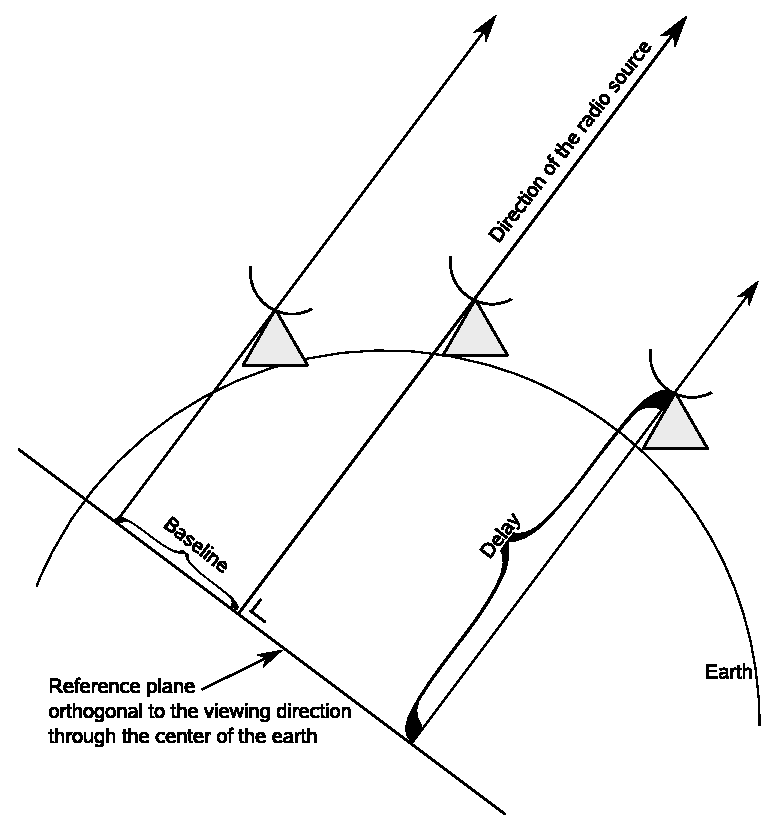
\includegraphics[width=.75\textwidth]
  {img/VLBI}
  \caption{Block diagram of the correlation.}
  \label{fig:correlation_diagram}
\end{figure}
\paragraph{Correlation}
Correlation is the process by which data from multiple telescopes is
collected and combined to measure the spatial Fourier components of
the image of the sky. The high data rates and the optimizations
complicate the process.

Assume that we are correlating the signal of two telescopes. First,
both signals are delayed to account for the different time at which
the signal arrives at the telescopes, see
Figure~\ref{fig:correlation_diagram}.  This process requires very
accurate timing information in the data and a very detailed model of
the geometry of the experiment. After the signals are properly
aligned, the signals are ready to be correlated. Correlation is a well
defined mathematical function~\cite{def_correlation} on two signals in
which the first signal is delayed with discrete steps and the integral
is computed of of the delayed signal multiplied with the second
signal. To increase the signal to noise ratio, the correlated signal
is averaged over a certain period of time. Typical averaging times lie
in the range of $0.25-4$ seconds.

For more than two stations, each station is correlated with itself
(auto-correlation) and every other station (cross-correlation). Note
that the complexity is quadratic in the number of telescopes.


%%% Local Variables:
%%% mode: latex
%%% TeX-master: "Ingrid"
%%% End:

\section{VLBI}\label{sec:vlbi}
\acomment{NGHK: Move to the introduction}{Recent Astronomical research
  studies the deep-sky (sources farther and farther away from us)
  which requires higher and higher angular resolution to capture all
  the details of the observed sources.  Increasing the size of a
  telescope dish increases the angular resolution of the image.
  However, it is difficult to build a moveable telescope dish with a
  size much larger than 100m.} Interferometry provides a possible
solution to \acomment{change}{this problem} as it combines the measurements of
several telescopes to simulate a dish of a size equivalent to the
maximal distance between the farthest telescopes on the plane
orthogonal to the viewing direction. Numerous arrays (groups of
telescopes) use this technique, e.g., the VLA (Very Large Array),
Lofar (Low-frequency array), the EVN (European VLBI Network) or the
VLBA (Very Large Baseline Array). Interferometry with telescopes that
are geographically very far apart is refered to as Very Large Baseline
Interferometry (VLBI). VLBI permits to build a virtual radio-telescope
with a dish of a size of the Earth. As the angular resolution of a
VLBI experiment depends on the maximal projected distance between two
radio-telescopes, VLBI achieves unsurpassed angular resolution with
the drawback of a relatively low sensitivity. Sensitivity is important
as it allows to detect fainter astronomical objects, increasing the
sensitivity is possible by adding more radio-telescopes or by
increasing the sample's resolution or the sampling rate, and thus
having more data gathered per telescope.

In order to get the final picture the signal gathered from the
radio-telescopes have to be correlated at a central place, the Joint
Institute for VLBI in Europe (JIVE), for correlation.  JIVE is
operating a dedicated hardware correlator~\cite{EVNCorrelator}.

The maximal capacity of this hardware correlator is 16 telescopes at a
data rate of 1Gbs each. The requirements on both the data streams and
the computing power are shown in Table~\ref{tab:speed}.

% \marginpar{NGHK: Check 16Mb/s in table}
\begin{table}
  \centering
  \begin{tabular}[c]{|l|l|l|l|l|l|}
    \hline
    Description & \# & \#  & data-rate & spect/prod & Tflops\\
    & telescopes & sub-bands & (Mb/s) &  & \\
    \hline
    \hline
    Fabric-demo &4 &2 &16 &32 &0.16\\
    1 Gb/s, full array  &16 &16 &1024 &16 &83.39\\
    future VLBI &32 &32 &4096 &256 &\verb|~|21457\\
    \hline
  \end{tabular}
  \caption{Network bandwidths and computing power needed for an {\it e}-VLBI
    experiment based on a XF architecture.}
  \label{tab:speed}
\end{table}

\paragraph{Correlation}\marginpar{NGHK: Split how/why correlation}
Correlation is the process by which data from multiple telescopes is
collected and combined to measure the spatial Fourier components of
the image of the sky.

Assume that we are correlating the signal of two telescopes. First,
both signals are delayed to account for the different time at which
the signal arrives at the telescopes, see
Figure~\ref{fig:correlation_diagram}. This process requires very
accurate timing information in the data and a very detailed model of
the geometry of the experiment. After the application of delay the
signals are properly aligned and the can be correlated.
Correlation~\cite{def_correlation} is mathematically defined as a
function on two signals in which \acomment{this is the mathematical
  definition}{the first signal is delayed with discrete steps and the
  integral is computed of the delayed signal multiplied with the
  second signal}. To increase the signal to noise ratio, the
correlated signal is averaged over a certain period of time. Typical
averaging times lie in the range of $0.25-4$ seconds.

For more than two stations, each station is correlated with itself
(auto-correlation) and every other station (cross-correlation). Note
that the complexity of the correlation is quadratic in the number of
telescopes, as it is linear in the number of baselines (telescope
pairs).

\paragraph{{\it e}-VLBI}
Traditionally, in VLBI, the data is recorded at the telescopes on disk
packs during an experiment. After the experiment the disks are shipped
to a central institute. There can be several weeks between the
experiment and the time when the correlated data becomes available.

Currently, JIVE is in the transition phase from traditional VLBI to
{\it e}-VLBI~\cite{szomoru-2004}. In an electronic VLBI ({\it e}-VLBI)
experiment, data from the telescopes is transferred directly over the
internet to JIVE, where it is streamed into the correlator in real
time. The data transport from the telescopes to JIVE goes over several
networks like local connections, paths provided by NRENs and the
G\'EANT backbone in Europe.

Transporting the data over the network has several advantages over a
traditional experiment. Obviously, the results of the experiments are
almost immediately available. This opens up the possibility to change
the course of an experiment based on earlier findings. Also, {\it
  e}-VLBI allows for real time analysis of the data and helps to
identify and resolve minor technical problems in the data collection
during the experiment.

Several experiments in the past have shown that real time {\it e}-VLBI
is possible. The EC funds the EXPReS project\footnote{EXPReS is made
  possible through the support of the European Commission (DG-INFSO),
  Sixth Framework Programme, Contract \#026642.}~\cite{EXPReS} which
aims at building a production-level {\it e}-VLBI instrument of upto 16
intercontinental telescopes connected in real-time to JIVE and
available to the general astronomy community.

%%% Local Variables:
%%% mode: latex
%%% TeX-master: "Ingrid"
%%% End:

\section{Software correlator}\label{sec:softwarecorrelation}
If the data in an {\it e}-VLBI experiment can be streamed over the
internet to JIVE, it can also be sent to another correlator. Within
\scarie, we are investigating the possibilities of a next generation
software correlator using a computing Grid. A similar attempt is
presented in \cite{deller-2007}. The advantages of a software
correlator over a new dedicated hardware correlator lie in its
flexibility and accuracy. The main advantage of a dedicated hardware
correlator is the greater performance. The flexibility of its
architecture allows the software correlator to change with the
individual needs of researchers. In fact, the first version of the
software correlator was developed to track the Huygens spacecraft
during its descent through the atmosphere of Saturn's moon Titan. Due
to the nature of this experiment, special requirements are put on the
correlator, which the current hardware correlator is not able to
provide.  Moreover, we expect that the costs of developing a software
correlator are much lower than the costs for a hardware correlator.

\begin{comment}
  The advance of general purpose computing is making software
  correlation a cost-effective solution for a range of applications.
\end{comment}

Currently, the software correlator is used in the production
environment for doing ftp-fringe tests. Since the EVN is an ad-hoc
array, the telescopes are reconnected before every VLBI-session. In
order to test the network, the telescopes observe a well known source
and transmit the data to JIVE where it is processed immediately. The
EVN ftp fringe tests provide quick feedback to the stations on their
performance.

Computationally the correlation is relatively inexpensive, in the
sense that it requires only few operations per transferred bytes.
However, due to the high data rates, the absolute number of clock
cycles required by the application is still extremely high.  Moreover,
the problem is quadratic in the number of telescopes participating in
the experiment since it is linear in the number of channel pairs that
have to be correlated. The huge need for networking and computing
power together with it's flexibility, makes a computing Grid an ideal
platform for this application.



\begin{figure}
  \centering
  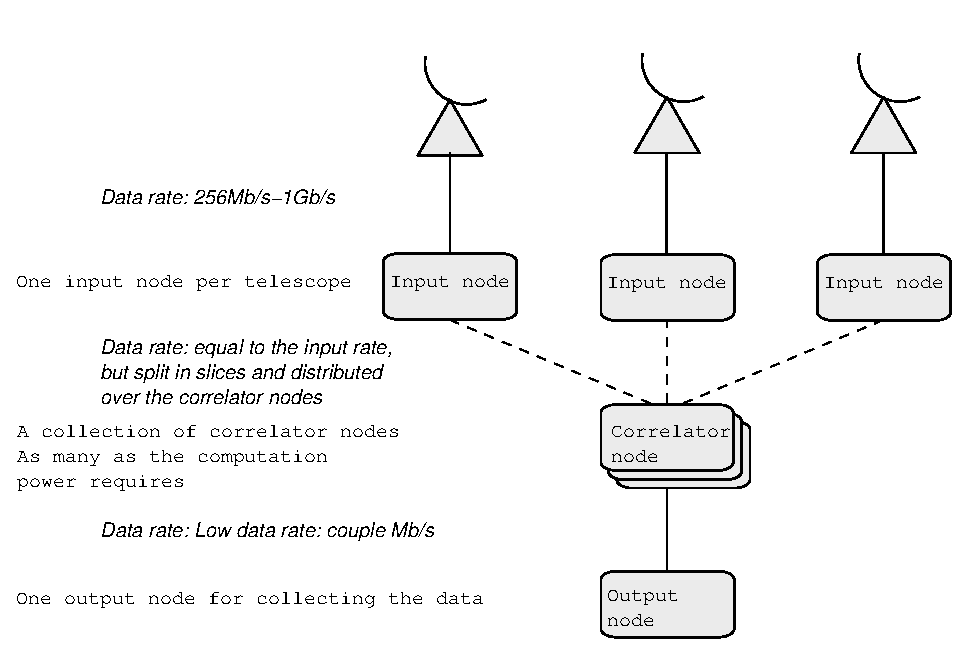
\includegraphics[width=.75\textwidth]
    {img/Network_correlator}
    \caption{Outline of the network connections between different
      components in the software correlator.}
  \label{fig:netw_corr}
\end{figure}


\subsection{Design}
In the software correlator, we split the computation in time slices.
These time slices are processed in parallel (see
Figure~\ref{fig:netw_corr}). The signal from a telescope is received
by a single so-called input node.  The input node sends slices of data
to one of the available correlator nodes. The correlator node receives
data from all telescopes for a certain time slice and performs the
correlation. The size of the output of the correlation is much smaller
than the input size and can be collected and stored by a single output
node.  There is a single manager node that assigns data to available
computing nodes.

\begin{comment}
  The software correlator is written in \verb~C++~ and uses several
  standard libraries like \verb~fftw~ \cite{FFTW05} for the fast
  Fourier transforms, \verb~mpich~ \cite{Gropp:1996:HPI} as the MPI
  implementation , \verb~GSL~ \cite{GSL} for cubic spline fitting and
  the standard template library.
\end{comment}

The manager node is the central node that controls the workflow of the
entire software correlator. It assigns time slices to available
correlator nodes and handles errors. After all time slices are
processed it terminates the software correlator.

The input node receives the data from a data stream, which can either
be a file, a TCP connection or directly from the dedicated hardware
used to record and play back the data. On request of the manager node,
it can extract the current time from the data stream or go to a
specified time. When the input node gets a request to send data for a
certain time slice to a correlator node, it seeks the right starting
sample in the input stream and sends the data to the correlator node.

The correlator node gets data for the same time slice from every input
node. First it, compensates for the fractional delay and performs the
phase rotation. These manipulations are not done on the input node
because they require floating point samples, hence the data stream
expands from 2 bits per sample to 32 bits or even 64 bits per sample,
which would require much more network bandwidth. After the fractional
delay correction and the phase rotation, the signal is ready to be
correlated.  The auto and cross correlation are then computed by
Fourier transforming the input signal and element-wise multiplying all
combination of telescope-pairs. These values are accumulated over a
certain period of time and the accumulated values are sent to the
output node.

The output node will receives the data from the correlator nodes,
sorts the data and stores it at a specified location.

%%% Local Variables:
%%% mode: latex
%%% TeX-master: "Ingrid"
%%% End:

%\input{data_flow.tex}
\section{Execution and deployment.}\label{sec:network}
In the context of \evlbi\ the software correlator can be executed in
two different operational modes that are: \emph{batch-execution} and
\emph{real-time}. Grids have a long history in running batch jobs and
grid-middleware is now doing a good job on this task. The execution of
real-time applications is much more complex; grid infrastructure and
middleware have to provide guarantees on the Quality of the Service to
insure successful execution of the job. Quality of Service management
in grids is still evolving rapidly. To experiment with these aspects
we are running \scarie\ on a research grid called DAS-3 and its
manageable network called StarPlane.

\subsection{Real-time and quality of service}
The term \emph{real-time} has many definitions in the computer science
community, in this paper we will consider that a \emph{real-time}
computation is a computation in which: \emph{the amount of buffering
  for an infinitely long experiment will only require a finite amount
  of buffers}. This is a formal way to define a process in which the
incoming data are "consumed" by the computation as fast as they are
generated. This definition also implies that once the application is
started the allocated "space" on the resources will be maintained
during the complete execution.

The main resources \scarie\ is using are: the network bandwidth, the
computation resource and the disk-space. Sharing of the computational
resource is now a well understood process and most of the time it is
part of the execution service that allocates the requested resources
and if all resources are acquired, it deploys and executes the
application.
%\begin{comment}
%\begin{figure}
%  \centering
%  \includegraphics[width=\textwidth]
%    {img/mapping.eps}
%    \caption{Left: An specific instaInce of an experiment. Right: The
%      resource set. Resource allocation and application scheduling
%      have to map the left side to the resources. }
%  \label{fig:mapping}
%\end{figure}
%\end{comment}
The simplest way to offer guaranteed service over a shared resource
can be done by restricting the access to only one user at a time. This
approach is used in the DAS-3 grid (based on SGE) in which an
allocated node is simply unusable by other users. Same principle could
be applied to the complete grid including its networks and other
resources. A more flexible approach consists in sharing the resource
under the arbitration of a third party that will insure that each
application is using only the allocated part of the resource. This is
the case with Layer-3 QoS for networks, or the Completely Fair Scheduler 
(per application CPU time allocation) combined with the Process Containers 
recently introduced into the Linux Kernel\cite{cfs}. In
a very general point of view all these technologies virtualize the
resource thus they permit to build on top of a real grid a complete
isolated environment based on user requirements.

\subsection{Running \scarie on \das3 and Starplane}
Networking performance and QoS management is one of the most
challenging aspects of \scarie.  The regular Internet Layer3 IP
routing based on the best-effort policy has a great flexibility but is
often slow and unpredictable; on the other hand, we have dedicated
\textit{lightpaths} as available in \textit{lambda
  Grids}~\cite{eslea-2007}, with their predictable
delays and throughputs offer good performances and a good basis to
offer Quality of Service. Giving end users access to dedicated
connection has been implemented in many of the current research and
education networks. The Dutch National Resarch and Education network
SURFnet is one of them.  This is used to deliver the data from the
radio-telescope to the computation center.

In \scarie\ having lighpaths between radio-telescopes and the
computation center is not sufficient to insure real-time
operation. \scarie\ also uses the network to distribute the
correlation. Therefore, a per application manageable network is then
required. The \das3\ supercomputer~\cite{das3} is composed of fives
clusters located in the Netherlands and connected by a photonic
network called StarPlane. The StarPlane project manages eight
wavelengths with the goal to build a network service that permits
\textit{an application-controlled photonic network and node-to-node
  traffic isolation}. The novelty of the StarPlane project lies in its
attempt to build a virtual network service at the lowest possible
networking layer: the photonic layer for the optical part and
ethernet-layer2 for the connection to the nodes. Another
property of StarPlane is that the photonic lightpath can dynamically
be reorganized to match the requirements of the user-application. By
using StarPlane, a complete virtual network over distributed cluster
sites can be build on demand. The lighpaths can also be re-organized
at run-time if the network load changes. For \scarie this allows us to
distribute the workload over several cluster locations while taking
profit of the high-bandwidth with a relative good QoS control over the
complete network domain.

\subsection{Benchmarks on DAS-3}
\scarie~ and StarPlane have parallel roadmaps. Hence the complete
approach cannot be tested yet. We have conducted correlator
performance tests using \das3. The current software correlator is
currently able to perform a 4x128Mbps\marginpar{NGHK: CHECK}
experiment at 20\% of the real-time speed using a total of 16 (quad
core 2.0Ghz cpu) nodes.

In parallel with the benchmarks of the correlator, we are also testing
the capabilities of StarPlane to do high performance traffic isolation
that is needed for real-time correlation. At the time of writing
StarPlane has implemented the service that allows a program to build
and allocate a lighpath between two clusters on demand. We tested this
feature by running two client-server applications transmitting data
between clusters.

The network traffic of the two applications is depicted in
Figure~\ref{fig:timing}.  At the start of the application, a request
for lighpath allocation is issued (arrow 1). After a while the
throughput drops because the second application starts sending data as
well (arrow 2).  As long as the lighpath is not ready (photonic
switching takes 10 minutes) the application is sending the traffic to
the default 1Gb/s ethernet route; when the lighpath is ready (arrow 3)
the traffic is rerouted to the lightpath.

\begin{figure}[ht]
  \centering
  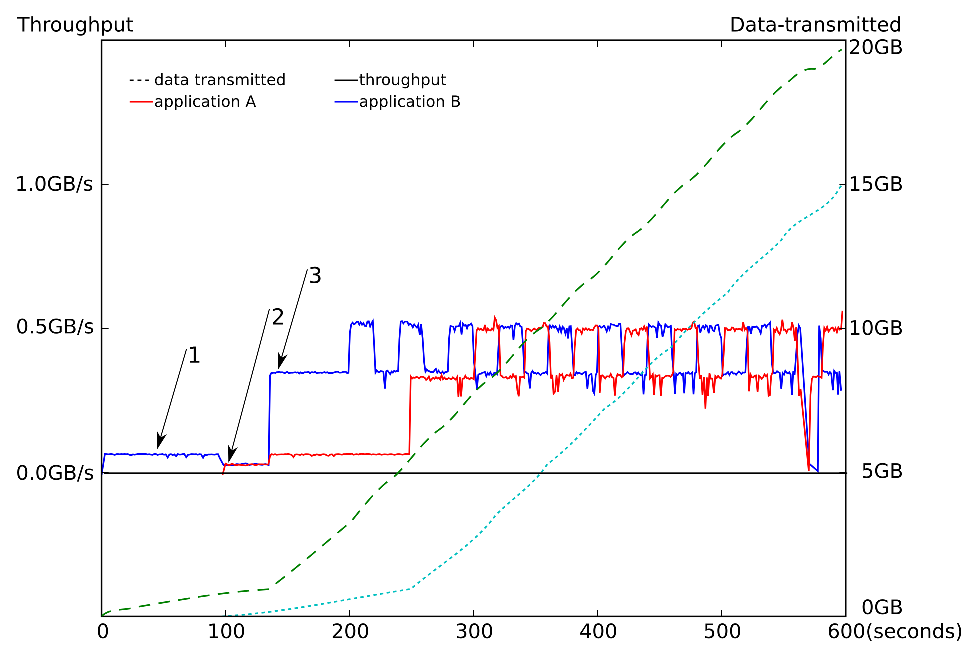
\includegraphics[width=\textwidth] {img/timing.eps}
  \caption{\label{fig:timing} Two application are started at time
    (arrow 1) and (arrow 2). The two applications have to share the
    1Gbps network bandwith. When a lighpath is allocated (arrow 3) the
    increase in performance is clearly visible.}
\end{figure} 

The results of this experiment are encouraging as they show that good
network performance can be obtained between several cluster
locations. Lighpath dynamic switching also permits to adapt the
photonic part of the network to the software correlation work load and
distribution.  Neverthless the results of this experiment also rise
questions, the secured lightpath is supposed to deliver reliably
"550MB/s" of throughput between a pair of clusters.  In
Figure~\ref{fig:timing} we can see a periodic artifact, the traffic
falling down to 300MB/s for few seconds, for which we have no
explanation. A second issue to investigate is that from time to time
the lighpath connectivity disapears entirely (e.g. at second 580). We
are currently working with Starplane team to understand and solve
these problems.


%%% Local Variables:
%%% mode: latex
%%% TeX-master: "Ingrid"
%%% End:

%\section{Benchmarks}\label{sec:benchmarks}

%%% Local Variables:
%%% mode: latex
%%% TeX-master: "Ingrid"
%%% End:

\section{Conclusion and future work}\label{sec:conclusion}
In the last year we laid the foundation for a flexible software
correlator based on distributed computing technologies. \scarie\ is
now useable for batch correlation and is used for ftp-fringe tests for
the EVN.

In order to reach our real-time correlation goal, we are collaborating
intensively with the StarPlane project to test new network
architectures for grids with guarenteed Quality of Services.

\paragraph{Future work}
Within \scarie\ and a related project FABRIC, which is a joint
research activity in the EXPR{\it e}S project, we are currently
improving and testing the software correlator. We still see
possibilities to improve the efficiency of the software correlator,
which we would like to investigate further.

On the batch processing aspect of \scarie\ we want to investigate how
resources can be added dynamically at runtime to accelerate the
computation. This include node joining and leaving as well as setting
up additional lighpaths to the new nodes.

On the real-time processing aspect, more work has to be done on the
traffic isolation features of the incoming networks as well as the
isolation provided by Starplane. 

\section{Acknowledgment}
\scarie\ is a joint research project between JIVE, the University of
Amsterdam and SARA funded by the Netherlands Organization for
Scientific Research (NWO).



%%% Local Variables:
%%% mode: latex
%%% TeX-master: "Ingrid"
%%% End:


% BibTeX users please use
\bibliographystyle{plain}
\bibliography{biblio}

%\ifodd\thepage
%\newpage
%\thispagestyle{empty}
%\centerline{\hfill}
%\fi
\end{document}

